\documentclass[tikz,border=0pt]{standalone}
\usepackage[T1]{fontenc}
\usepackage[utf8]{inputenc}
\usepackage{helvet}
\renewcommand{\familydefault}{\sfdefault}
\usepackage{amsmath,textcomp}
\usepackage{pgfplots}
\pgfplotsset{compat=1.18}
\usetikzlibrary{plotmarks}
\definecolor{Bzero}{HTML}{4D4D4D}
\definecolor{Btwo}{HTML}{0072B2}
\definecolor{Bthree}{HTML}{E69F00}
\definecolor{Bfour}{HTML}{CC79A7}
\definecolor{Mcal}{HTML}{D55E00}
\definecolor{Nofat}{HTML}{009E73}
\definecolor{Ink}{HTML}{202020}
\definecolor{Muted}{HTML}{666666}
\definecolor{Grid}{HTML}{DDDDDD}
\pgfplotsset{iraxis/.style={scale only axis,axis lines*=left,
  axis line style={line width=.45pt,Ink},tick style={line width=.45pt,Ink},
  tick align=outside,tick pos=left,major tick length=1.4mm,
  font=\fontsize{7.5}{8.5}\selectfont,
  tick label style={font=\fontsize{7}{8}\selectfont},
  xticklabel={\pgfmathprintnumber[fixed,precision=3,assume math mode=true]{\tick}},
  yticklabel={\pgfmathprintnumber[fixed,precision=3,assume math mode=true]{\tick}},
  label style={font=\fontsize{7.5}{8.5}\selectfont},
  scaled ticks=false,unbounded coords=jump,
  ymajorgrids=true,xmajorgrids=false,grid style={Grid,line width=.35pt},
  enlargelimits=false,clip=true}}
\newcommand{\unitmd}{\textmu m\texttwosuperior/ms}
\begin{document}
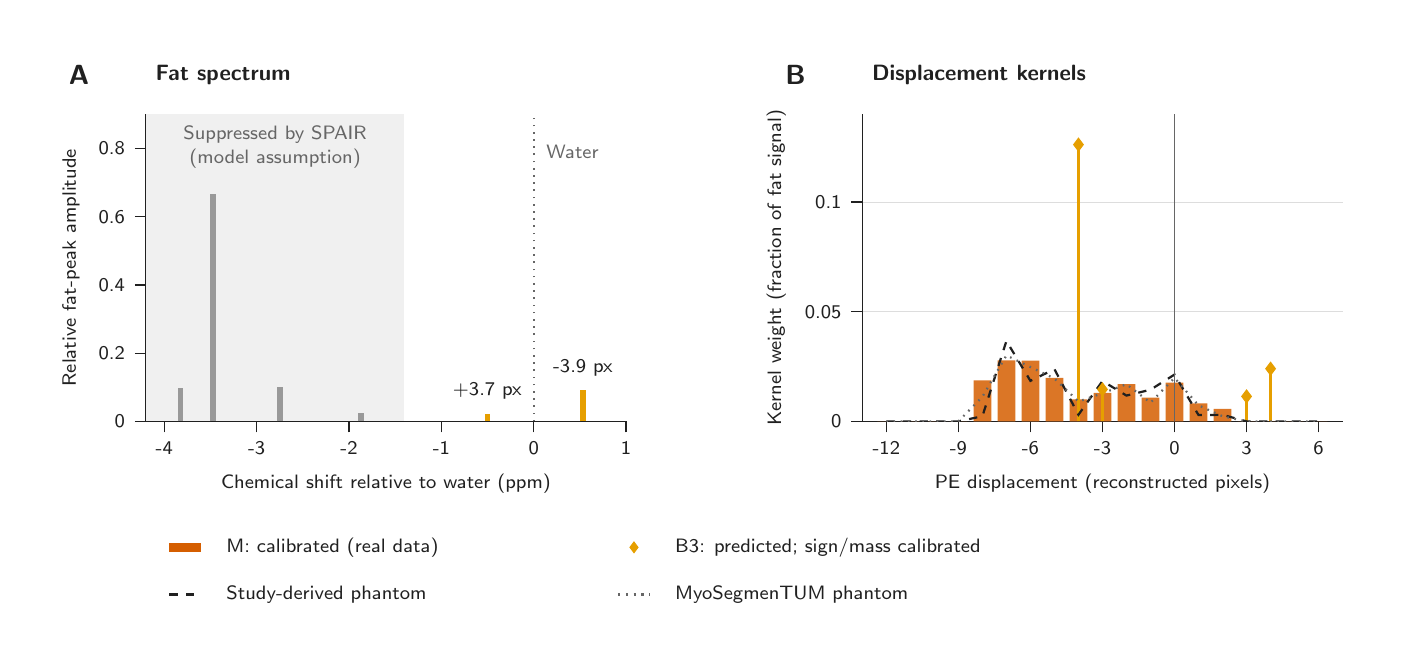
\begin{tikzpicture}[x=1mm,y=1mm,font=\fontsize{7.5}{8.5}\selectfont,text=Ink]

\path[use as bounding box] (0,0) rectangle (174,75);
\node[anchor=west,font=\fontsize{10}{11}\selectfont,font=\bfseries\fontsize{10}{11}\selectfont] at (4,69) {A};
\node[anchor=west,font=\fontsize{8}{9}\selectfont,font=\bfseries\fontsize{8}{9}\selectfont] at (15,69) {Fat spectrum};
\begin{axis}[iraxis,at={(15mm,25mm)},anchor=south west,width=61mm,height=39mm,xmin=-4.2,xmax=1,ymin=0,ymax=.9,xtick={-4,-3,-2,-1,0,1},xlabel={Chemical shift relative to water (ppm)},ylabel={Relative fat-peak amplitude},ymajorgrids=false]
\path[fill=black!6] (axis cs:-4.2,0) rectangle (axis cs:-1.4,.9);
\addplot[no marks,line width=.6pt,color=black!40,line width=2pt] coordinates {(-3.825,0) (-3.825,0.09733)};
\addplot[no marks,line width=.6pt,color=black!40,line width=2pt] coordinates {(-3.4711,0) (-3.4711,0.66598)};
\addplot[no marks,line width=.6pt,color=black!40,line width=2pt] coordinates {(-2.7462,0) (-2.7462,0.0996)};
\addplot[no marks,line width=.6pt,color=black!40,line width=2pt] coordinates {(-1.8679,0) (-1.8679,0.02328)};
\addplot[no marks,line width=.6pt,color=Bthree,line width=2pt] coordinates {(-0.5026,0) (-0.5026,0.02287)};
\node[above,font=\fontsize{7}{8}\selectfont] at (axis cs:-0.5026,0.03487) {+3.7 px};
\addplot[no marks,line width=.6pt,color=Bthree,line width=2pt] coordinates {(0.5323,0) (0.5323,0.09095)};
\node[above,font=\fontsize{7}{8}\selectfont] at (axis cs:0.5323,0.10295) {-3.9 px};
\addplot[no marks,line width=.6pt,color=Muted,dotted] coordinates {(0,0) (0,0.9)};
\node[font=\fontsize{7}{8}\selectfont,text=Muted] at (axis cs:-2.8,.84) {Suppressed by SPAIR};
\node[font=\fontsize{7}{8}\selectfont,text=Muted] at (axis cs:-2.8,.77) {(model assumption)};
\node[anchor=west,font=\fontsize{7}{8}\selectfont,text=Muted] at (axis cs:.03,.79) {Water};
\end{axis}
\node[anchor=west,font=\fontsize{10}{11}\selectfont,font=\bfseries\fontsize{10}{11}\selectfont] at (95,69) {B};
\node[anchor=west,font=\fontsize{8}{9}\selectfont,font=\bfseries\fontsize{8}{9}\selectfont] at (106,69) {Displacement kernels};
\begin{axis}[iraxis,at={(106mm,25mm)},anchor=south west,width=61mm,height=39mm,xmin=-13,xmax=7,ymin=0,ymax=.14,xtick={-12,-9,-6,-3,0,3,6},xlabel={PE displacement (reconstructed pixels)},ylabel={Kernel weight (fraction of fat signal)}]
\addplot[ybar,bar width=2.25mm,fill=Mcal!85,draw=none] coordinates {(-12,0.0) (-11,0.0) (-10,0.0) (-9,0.0) (-8,0.018671805683536085) (-7,0.027797849053325236) (-6,0.027650407864794585) (-5,0.01984520412078774) (-4,0.010006110735662859) (-3,0.012945746632377794) (-2,0.01693280040783669) (-1,0.010847626458193671) (0,0.017617146902508592) (1,0.008165867446993403) (2,0.005670528941412148) (3,0.0) (4,0.0) (5,0.0) (6,0.0)};
\addplot[no marks,line width=.6pt,color=Bthree,line width=.8pt] coordinates {(-4,0) (-4,0.126163549097)};
\addplot[only marks,mark=diamond*,mark size=2.3pt,color=Bthree,mark options={fill=Bthree,draw=Bthree},] coordinates {(-4,0.126163549097)};
\addplot[no marks,line width=.6pt,color=Bthree,line width=.8pt] coordinates {(-3,0) (-3,0.014597913546)};
\addplot[only marks,mark=diamond*,mark size=2.3pt,color=Bthree,mark options={fill=Bthree,draw=Bthree},] coordinates {(-3,0.014597913546)};
\addplot[no marks,line width=.6pt,color=Bthree,line width=.8pt] coordinates {(3,0) (3,0.0113756708841)};
\addplot[only marks,mark=diamond*,mark size=2.3pt,color=Bthree,mark options={fill=Bthree,draw=Bthree},] coordinates {(3,0.0113756708841)};
\addplot[no marks,line width=.6pt,color=Bthree,line width=.8pt] coordinates {(4,0) (4,0.0240139607204)};
\addplot[only marks,mark=diamond*,mark size=2.3pt,color=Bthree,mark options={fill=Bthree,draw=Bthree},] coordinates {(4,0.0240139607204)};
\addplot[no marks,line width=.6pt,color=Ink,dashed,line width=.8pt] coordinates {(-12,0) (-11,0) (-10,0) (-9,0) (-8,0.00233456306343) (-7,0.0366457249854) (-6,0.018478698362) (-5,0.0237874011647) (-4,0.00302932003251) (-3,0.0183977941921) (-2,0.011762751469) (-1,0.0144315131097) (0,0.0213409416042) (1,0.00287643729518) (2,0.00298647256869) (3,0) (4,0) (5,0) (6,0)};
\addplot[no marks,line width=.6pt,color=Muted,dotted,line width=.8pt] coordinates {(-12,0) (-11,0) (-10,0) (-9,0) (-8,0.0112183639007) (-7,0.0300717632858) (-6,0.0247881669415) (-5,0.0195495232428) (-4,0.00907190974152) (-3,0.0128084403318) (-2,0.0169471376755) (-1,0.00851050695656) (0,0.0198411856773) (1,0.00729503529968) (2,0.00232990643241) (3,0) (4,0) (5,0) (6,0)};
\addplot[no marks,line width=.6pt,color=Muted,line width=.4pt] coordinates {(0,0) (0,0.14)};
\end{axis}
\draw[Mcal,line width=3pt] (18,9)--(22,9);
\node[anchor=west,font=\fontsize{7}{8}\selectfont,] at (24,9) {M: calibrated (real data)};
\draw[color=Bthree] plot[mark=diamond*,mark size=1.9pt,mark options={fill=Bthree,draw=Bthree}] coordinates {(77,9)};
\node[anchor=west,font=\fontsize{7}{8}\selectfont,] at (81,9) {B3: predicted; sign/mass calibrated};
\draw[Ink,dashed,line width=.8pt] (18,3)--(22,3);
\node[anchor=west,font=\fontsize{7}{8}\selectfont,] at (24,3) {Study-derived phantom};
\draw[Muted,dotted,line width=.8pt] (75,3)--(79,3);
\node[anchor=west,font=\fontsize{7}{8}\selectfont,] at (81,3) {MyoSegmenTUM phantom};
\end{tikzpicture}
\end{document}
